THz Spectroscopy performed in the time-domain also known as THz Time Domain Spectroscopy (THz-TDS) is a spectroscopy technique based on the optical excitation of photoconductive antennas. This type of THz spectroscopy was made possible through the development of the femtosecond laser since the photoconductive antennas require ultrafast laser pulses for the generation of broadband THz radiation. A more elaborate description of the generation and detection mechanisms is presented in sections \ref{sec:thz-generation} and \ref{sec:thz-detection}. Additionally, compared to other spectroscopy methods such as Fourier-transform spectroscopy THz-TDS has the advantage that both the amplitude and phase of the radiation can be measured since the measurement takes place in the time-domain. Another property of THz-TDS is that the radiation employed is non-ionizing which possibly enables its use in areas not suited for e.g. x-ray spectroscopy. In addition, a wide range of materials are transparent in the THz energy range so that underlying layers can be probed without physically altering the sample \cite{Horlick68, Jepsen2011}.
% add that it's useful in our case, for device characterization. Jepsen
\section{Generation}
\label{sec:thz-generation}
There exists several techniques based on different mechanisms which can be employed in the TDS setups for the generation of THz radiation \cite{Jepsen2011}. Specifically in this work we use photoconductive conductive antennas for this purpose. 

\begin{figure}[H]
    \centering
    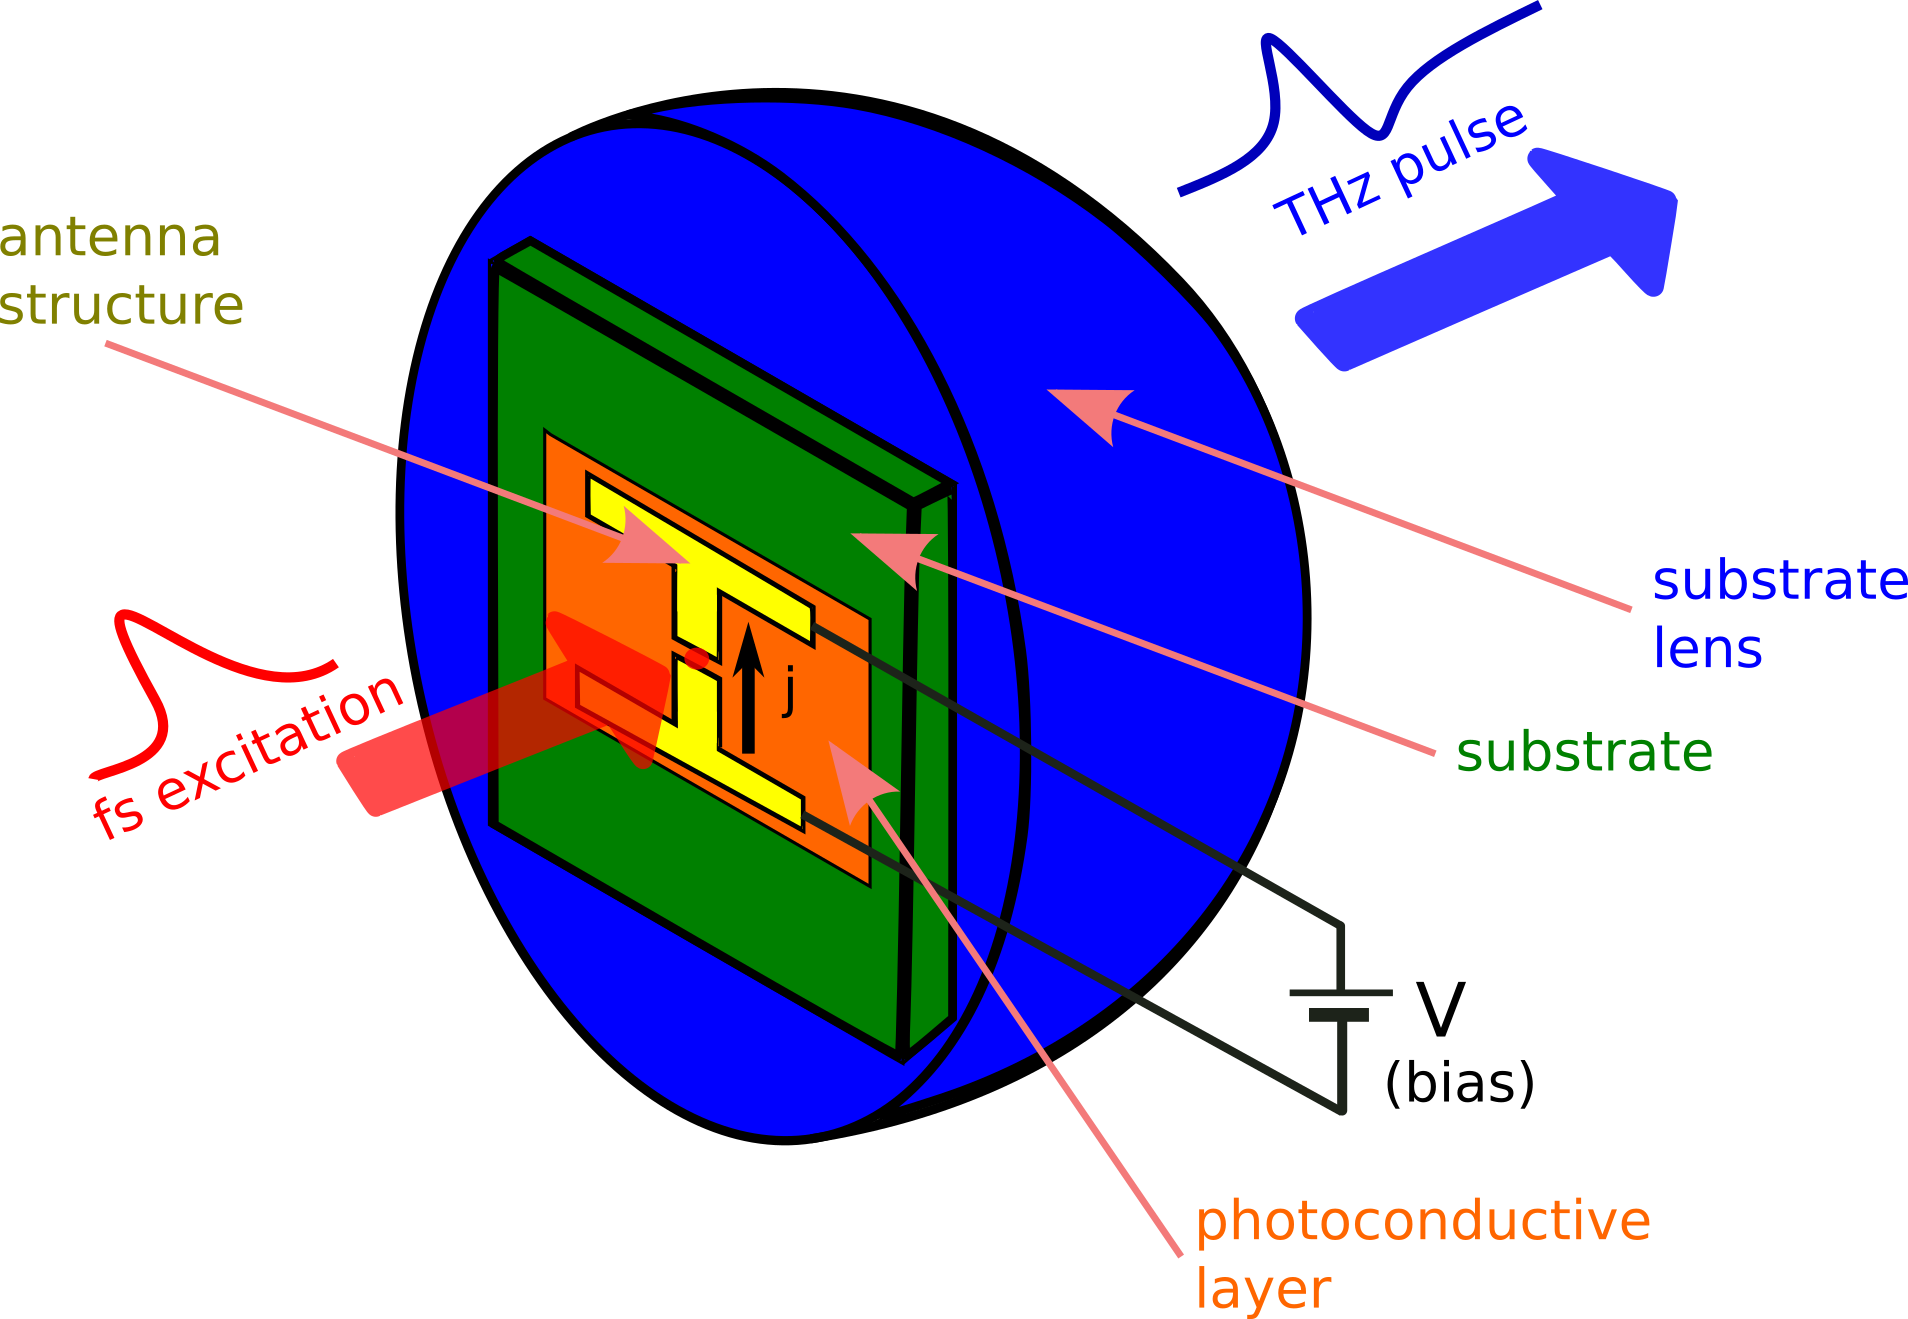
\includegraphics[scale=0.5]{images/2_chapter02/PCA.png}
    \caption{Sketch of a photoconductive antenna. The incoming laser pulse generates free charge carriers in the semiconductor substrate. The free charge carriers move due to the applied voltage so that a current flows between the anode and cathode. This high acceleration of the charge carriers causes them to emit radiation in the THz range. The silicon lens(shown in blue) helps couple the radiation into free space from the substrate.}
    \label{fig:PCA}
\end{figure}

\section{Detection}
\label{sec:thz-detection}
